\part{Naissance d’un vrac numérique au Musée des Arts Décoratifs}

\chapter{Le service Archives du MAD}

Dans tout domaine d’étude, parler de réorganisation implique une bonne compréhension de la genèse du cas proposé à l’appréciation. En archivistique, cela revient à mettre l’accent sur les différents procédés qui ont conduit à cette masse non organisée. Avec l’avènement du numérique, l’abondance de données disponibles constitue un nouveau terrain de jeu de nouvelles réflexions\footnote{\cite{bermes-charpier-stutzmann-2026}. p. 3.}, notamment dans le domaine du traitement archivistique. C’est à partir de cette production croissance que les documents subissent une dislocation des liens qui existent entre eux, ce qui rend difficile leur repérage et leur accessibilité.

Pour comprendre l’apparition du vrac numérique dans les institutions patrimoniales, il faut savoir qu’il ne constitue pas un phénomène isolé. Il se situe dans la plupart des cas dans l’histoire institutionnelle, organisationnelle impactant la manière dont les documents sont produits, utilisés et conservés. C’est dans cette perspective que l’étude des archives d’exposition revient à situer la fonction Archive dans l’écosystème documentaire du musée. Ceci dans le but de comprendre les bases de la gestion documentaire. 

La mise en avant de la fonction Archives au musée suit la progression logique de l’histoire du musée. Pour la comprendre, il est important pour nous de remonter à la genèse de l’Union centrale des beaux-arts appliqués à l’industrie, en abrégée UCBAAI, de la Bibliothèque-Archives-Documentation (BAD) de l’institution.

Le chapitre est réparti en trois temps. Il se propose d’abord de revenir sur la construction d’une vocation documentaire au musée des arts décoratifs, ceci dans l’optique de présenter la production documentaire comme une ambition qui se situe dans le contexte historique de l’institution. Ensuite, il fait une présentation du service archives et de la fonction qui en découle. Enfin, il présente les catégories d’archives dont il a la charge.


\section{Construction d’une vocation documentaire}

Dès la création de l’Union centrale des beaux-arts appliqués à l’industrie, la documentation apparaît dans le but de soutenir la création artistique, la formation des artisans et la promotion des savoirs. Cette démarche prend plus de sens avec la création d’une bibliothèque spécialisée, constituant un véritable outil de recherche et de transmission des savoirs. En outre, la documentation est la résultante des activités bien anciennes.
 

\subsection*{Création de l’Union centrale et l’ambition du « beau dans l’utile »}

Fondée en 1863 sous la présidence d’Édouard Guichard, l’Union centrale des beaux-arts appliqués à l’industrie joue un rôle dans l’histoire du pôle Archives. En 1882, elle devient l’Union centrale des arts décoratifs (UCAD). L’association naît dans un environnement marqué par les transformations industrielles du XIXe siècle et par les débats autour de la place de l’art dans la production manufacturière. Face aux progrès industriels observés notamment en Angleterre, ses fondateurs souhaitent promouvoir une meilleure articulation entre création artistique et production industrielle française. L’objectif affiché est alors \enquote{d’entretenir en France la culture des arts qui poursuivent la réalisation du beau dans l’utile}\footnote{\cite{brunhammer-1992}. p. 11.}. Puis, en 2004, elle devient les Arts Décoratifs et en 2018 musée des arts Décoratifs selon le rapport d'activités de 2018\footnote{\cite{JP801-rapports}. p. 14-15.}. Elle œuvre depuis lors pour la reconnaissance des arts décoratifs, la valorisation du statut des artisans décorateurs, des ouvriers, ainsi que pour l’intégration de l’art vivant au sein des musées\footnote{\cite{mad-depuis-1864}}.

Cette ambition ne repose pas seulement sur l’enrichissement des collections d’objets. Elle fait également référence à la création d’outils permettant leur étude et leur diffusion auprès des artistes, des artisans, des chercheurs et des industriels. C’est dans ce contexte que la Bibliothèque de l’UCAD apparaît comme l’un des éléments fondamentaux de la gestion documentaire de l’institution. Sa création ne représente pas un simple support administratif, mais l’un des piliers cardinaux du projet institutionnel : associer le beau à l’utile pour former les artisans, guider les industriels et stimuler la création contemporaine.


\subsection*{La bibliothèque comme instrument de documentation, de formation et de recherche}

Le désir d’allier le « beau dans l’utile », porté par l’Union centrale des beaux-arts appliquées à l’industrie ne concerne pas seulement la constitution des collections d’œuvres ou l’organisation d’expositions. Il consiste aussi en la mise à disposition de ressources documentaires destinées à faciliter l’accès à la connaissance aux acteurs du développement des arts décoratifs, à l’instar des artistes, des designers, des artisans, des industriels et des chercheurs. Au moment où, dans les années 1791 dans le monde, États disposent déjà d’un espace à caractère d’une vaste usine de reproductions destinée à fournir des modèles à l’école et à l’atelier, la France décide de se mêler au jeu et s’atteler à une nouvelle dynamique mondiale\footnote{\cite{A3-4-1887}. p. 3.}.

C’est dans cet élan que la bibliothèque est créée en 1864. Installée place des Vosges, à  quelques mètres du musée des modèles, qui constitue les ateliers des industriels\footnote{\cite{mad-histoire-bibliotheque}}, elle est pensée comme un  lieu de formation et d’inspiration  pour les ouvriers afin d’éduquer leur goût et de développer leur créativité tout en permettant aux industriels d’arts parisiens de conserver leur suprématie dans les arts décoratifs\footnote{\cite{mad-histoire-bibliotheque}}. À cet effet, la bibliothèque n’est pas un simple lieu de conservation de livres, elle constitue : un espace éducatif, un projet culturel pour l’Union centrale. L’objectif est de créer une atmosphère d’apprentissage et de motivation, de concentration pour les différents acteurs. Elle est la combinaison de livres didactiques et de ressources héritées des fonds d’ateliers des industriels fondateurs.  Elle devient le levier de transmission et de diffusion des savoirs.\\[0.2cm]

La bibliothèque poursuit, quelques années plus tard sa vocation et se développe peu à peu. Avec l’avènement en 1882 de l’Union centrale des arts décoratifs, son emplacement change et, à cela s’ajoute un nouveau type de public, à des savoirs les étudiants, ce qui favorise l’accroissement des collections. En 1887, le conservateur Alfred de Champeaux dans l’optique d’organiser une collection iconographique s’allie à un donateur et membre du conseil d’administration du musée\footnote{\cite{mad-histoire-bibliotheque}}. Ce qui est à l’origine du plan de classement  qui optimise l’identification des ressources et favorise leur exploitation par les lecteurs. Cette évolution s’inscrit dans la volonté constante du musée de structurer l’information, ce qui prépare progressivement une politique documentaire globale au sein de la bibliothèque.

Au-delà de sa notoriété de lieu de conservation des livres et de lieu d’apprentissage, la bibliothèque constitue tout autant un espace de stockage des documents. Plusieurs fonds lui sont attribués, comme les fonds des créateurs, une partie des fonds de historique de l’UCAD.


\section{Présentation du service Archives}

La mise en place d'un service dédié aux archives dans les institutions n'est pas le fruit du hasard : elle résulte de volonté d'encadrer les règles de gestion des documents afin de garantir la conservation à long terme du patrimoine. Au MAD, elle procède de plusieurs réflexions sur la question et la volonté d'une protection pérenne du patrimoine culturelle dont il est le garant.

\subsection*{Émergence progressive de la fonction archives}

Les préoccupations sur les archives se ressentent au musée depuis le XIXe siècle. Vers la fin du XXe siècle, plusieurs situations et acteurs jouent un rôle majeur dans leur considération. L’une des figures emblématiques est Yolande Amic, conservatrice au musée des Arts décoratifs de 1963 à 1976. Elle produit tout au long de cette période des catalogues d’exposition et œuvre à la conduite d’une politique patrimoniale où la recherche documentaire et la présentation muséographique sont associées. En 1969, elle fonde le Centre de création industrielle (CCI) au sein duquel elle met en place une politique documentaire centrée sur la recherche, la collecte et la diffusion des savoirs techniques et industriels\footnote{\cite{siguret-repertoire-2001}. p. 2.}. Elle est l’une des premières personnes à s’intéresser aux archives historiques de l’institution\footnote{\cite{siguret-repertoire-2001}. p. 2.}. Désireuse d’apporter une structuration aux archives de l’UCAD, elle se lance dans les mêmes années dans la mission d’inventorier et classer les fonds.

Plusieurs personnalités vont s'inscrire dans la lignée de Yoland Amic au cours des années 1990. 1994 lancée, François Mathon, directeur adjoint du musée, porte un intérêt pour les archives produites par les services administratifs\footnote{\cite{krezidou-2021}. p. 23.}. Il met en place un plan de classement au sein de  l’UCAD, qui n'est jamais respectée\footnote{\cite{krezidou-2021}. p. 23.}.\\[0.2cm]

En 1997, la conservatrice Guillemette Delaporte réalise un état des lieux des archives et des différents espaces de stockage. Elle relève deux problématiques : la  consultation difficile des archives du fait de leur localisation dispersée et d’une absence de gestion centralisée\footnote{\cite{delaporte-1997}. p. 2.}.  Notons qu'à cette période, une partie des archives institutionnelles de l’UCAD fait l’objet d’une élimination, tandis que l’autre est versée à la bibliothèque. Malgré ce versement partiel, la bibliothèque est leur seul lieu de conservation : les archives demeurent réparties entre les différents services, selon les activités et les besoins de chacun\footnote{\cite{delaporte-1997}. p. 2.}. Grâce à leurs chantiers respectifs, Amic, Mathon et Delaporte contribuent à une prise de conscience sur la valeur des archives en tant que mémoire de l'institution.

En 1997, naît le désir de consacrer un service dédié aux archives. Dans le document préliminaire sur les archives, il est mentionné que l’idée principale de la création d’un tel service est de faciliter la centralisation et l’accès aux documents par tous. L'amorce de cette réflexion traduit la volonté de structurer la gestion des archives et de préserver la mémoire de l’UCAD.


En 2000, avec l’arrivée à la tête des musées de Béatrice Salmon\footnote{\cite{mad-depuis-1864}}, une nouvelle stratégie organisationnelle est mise en œuvre. Celle-ci se matérialise en 2001 par l’identification et l'harmonisation des services de l’inventaire, de la restauration et de la conservation préventive, des expositions, des publics, ainsi que la création d’une régie pour l’ensemble de l’institution\footnote{\cite{dion-histoire-bad-2026}}. C'est la prise de poste de Sophie Durrleman en tant que Directrice générale qui marque une transformation de l’Institution, tant sur le plan organisationnel que sur celui de ses implantations, avec la conduite de travaux et le déménagement des services. En effet, cette période correspond à la rénovation du musée, la réouverture de la bibliothèque et, la réinstallation des Ateliers du Carrousel\footnote{\cite{mad-depuis-1864}}. Cette dernière étant longtemps rattachée à la Direction de la Conservation, qui réunis à cette époque les musées (musée des arts décoratifs, de la mode et du Textile, de la Publicité et de Nissim de Camondo)\footnote{Voir annexe~\ref{annexe:organigramme-2000} à la page~\ref{annexe:organigramme-2000}.}, cette organisation permet la mise en œuvre de moyens transversaux au service des trois piliers fondateurs de son identité, à savoir les musées, la bibliothèque et l’enseignement\footnote{\cite{dion-histoire-bad-2026}}. Ces moyens répondent donc aux besoins d’une direction opérationnelle\footnote{Voir le rapport d’activité de 2001, p. 47, \cite{JP801-rapports}.}.

Comme nous l’avons mentionné dans nos propos précédents, l’analyse archivistique menée par  la conservatrice Yolande Amic est une étape déterminante dans la reconnaissance et l’affirmation du besoin fonction Archives au musée. En 2001, Florence Siguret décide de poursuivre les travaux de la conservatrice en apportant une révision du système de classification dans le but de concevoir un instrument de recherche pour le fonds de l’UCAD. Elle opte pour un plan de classement thématique avec une cotation alphanumérique\footnote{\cite{krezidou-2021}. p. 23.}.

Quelques années plus tard, la fonction Archives s’affirme pleinement dans la structure et le fonctionnement progressif du musée, ce qui marque une étape importante dans l’organisation et la préservation de la mémoire institutionnelle.

Malgré la présence d’un instrument de structuration et de recherche dédié à une partie des archives, la question de leur organisation reste sans réponse globale. En 2012, alors que les problématiques restent inchangées, ce sont les archives publiques qui captivent l’attention. En effet, a reconnaissance d’utilité publique de l’association lui impose une gestion réglementée de ses archives dites publiques\footnote{Conformément à l'article L211-4, \cite{code-patrimoine-legislative} .}. De ce fait, l'institution doit se doter d'outils pour faciliter leur gestion quotidienne\footnote{\cite{bauer-archives-publiques-2012}. p. 6.}.

\subsection*{L’année 2014 : un tournant décisif pour les archives}

L’année 2014 symbolise la concrétisation officielle et matérielle de la fonction Archives, ce qui se caractérise par la mise en place d’une mission transversale sur les archives conservées par l’institution\footnote{Rapport d’activité 2014, p. 78-79, \cite{JP801-rapports}.}. Rappelons que, l’association des Arts décoratifs est reconnue d’utilité publique par le décret du 15 mai 1882, et a pour principal objectif d’entretenir et de développer en France la culture des arts qui poursuivent la réalisation du beau dans l’utile\footnote{\cite{mad-statuts-2023}, art. 1.}.

Elle est liée à l’État par une convention qui lui confère une mission de service public de garde, d’entretien, de gestion, de mise en valeur, d’enrichissement, d’étude et de présentation au public des collections muséographiques et des documentations nationales\footnote{\cite{mad-statuts-2023}, art. 1.}.

C’est dans ce contexte d’obligation légale qu’en 2014 avec la collaboration du ministère de la Culture, le recrutement d'une responsable des archives est effectué au mois de mai en la personne d’Élise Barzan. Cette action a pour principal objectif de promouvoir la coordination de la collecte, du traitement et de la valorisation des archives produites par l’ensemble de l’association. Cette mission transversale de l’archiviste ne concerne pas seulement le classement des fonds déjà existants; elle vise à initier la mise en place d’une politique d’archivage au sein de l’institution.

Le rapport d’activité de 2014 fait l’état de la mise en œuvre de la politique d’archivage. Il stipule que plusieurs actions sont menées telles que : la rédaction d’une charte formalisant les principes de gestion documentaire, la définition des modalités de traitement et d’archivage, et la mise en place d’un réseau de collaboration avec la mission des Archives du ministère de la Culture et le réseau de professionnels \enquote{Archives en musées}\footnote{Rapport d’activité 2014, p. 78-79, \cite{JP801-rapports}.}, ainsi que le renforcement des liens avec les Archives nationales.

Pour mobiliser l’ensemble des producteurs, l’idée est de nommer dix-neuf correspondants archives représentant les différentes directions et services des Arts décoratifs. Leur mission consiste à relayer la politique d’archivage à l’ensemble de leurs équipes et à faciliter l’application des pratiques en matière de gestion documentaire\footnote{Rapport d’activité 2014, p. 78-79, \cite{JP801-rapports}.}. La valorisation des fonds entraîne une augmentation des consultations comme les statistiques du rapport d’activités permettent de le constater.

\begin{figure}[H]
	\centering
	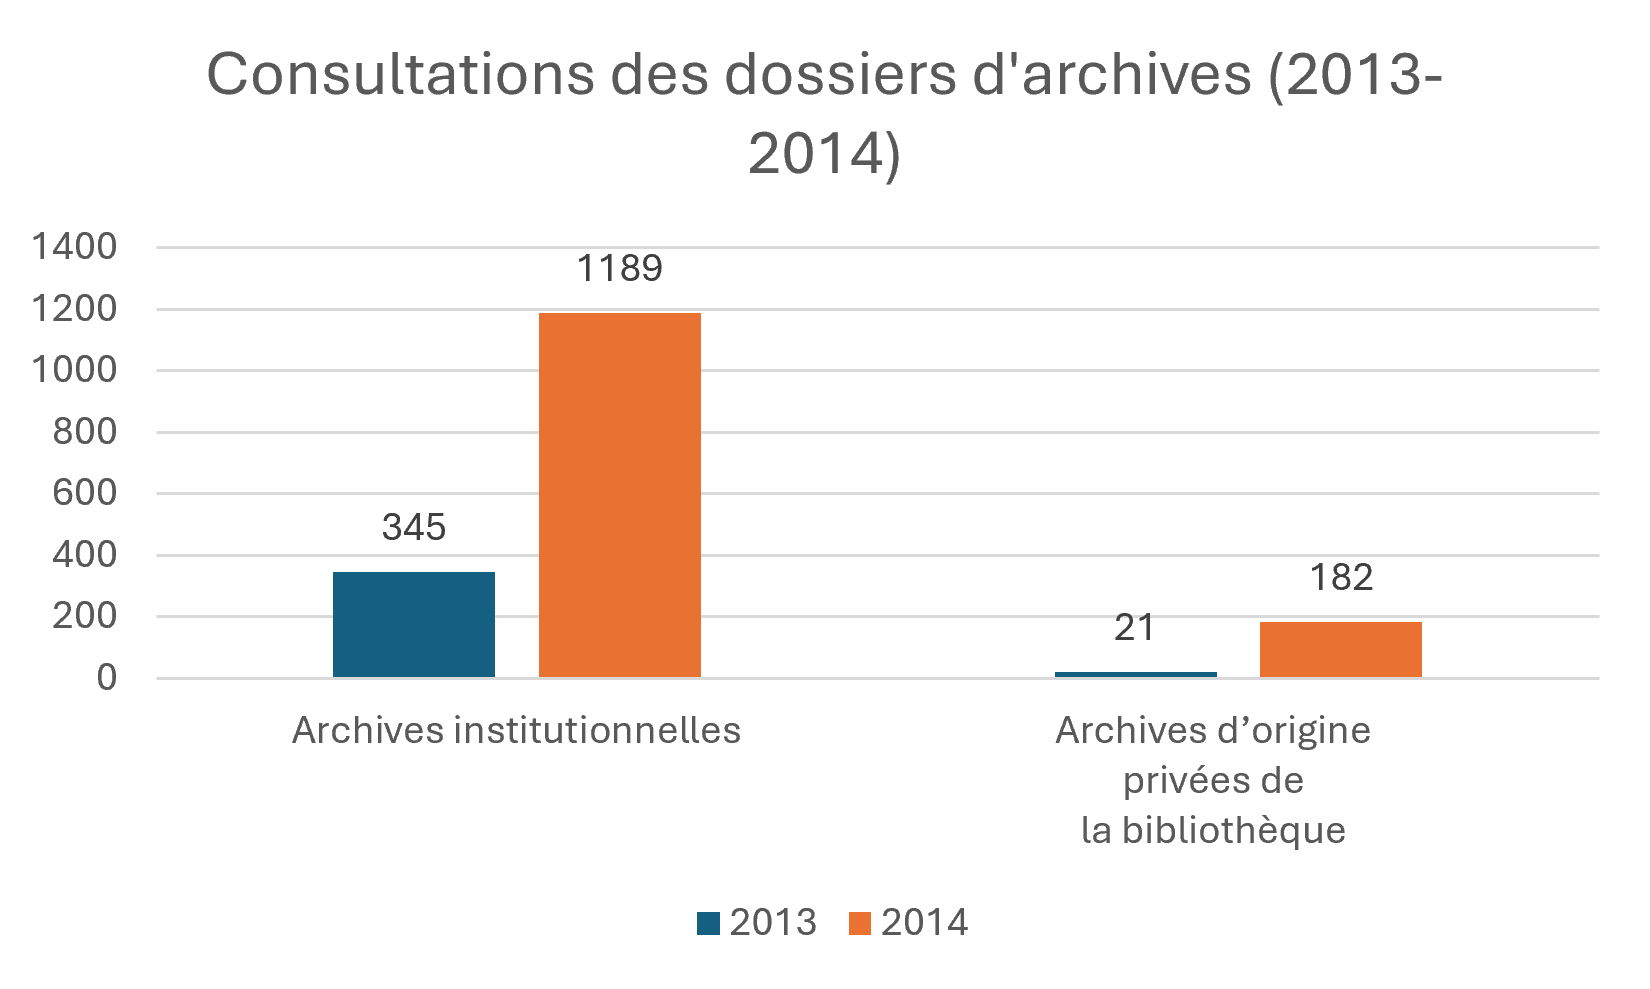
\includegraphics[width=0.8\textwidth]{Images/Consultation.png}
	\caption{Évolution du nombre de consultation des dossiers d'archives entre 2013 et 2014}
	\label{fig:Consultation}
\end{figure}

En 2013, 345 dossiers d’archives institutionnelles et 21 dossiers d’archives privées de la bibliothèque sont consultés, contre 1189 dossiers d’archives institutionnelles et 182 dossiers d’archives privées, en 2014. Cette forte augmentation représente plus de 270 ~\% du nombre de dossiers communiqués\footnote{Figure de statistique du nombre de consultation entre 2013-2014}. Le nombre total des lecteurs ayant consultés les archives en salle de lecture est également en hausse puisque sont dénombrés, 92 lecteurs en 2014 contre 85 en 2013.


\subsection*{La poursuite d’un renforcement de compétences}

Après les années 2018, principalement denses en matière de versement d’archives par les services de l’institution, l’année 2019 marque la transition, du fait du départ de l’archiviste. On note un versement important, de la direction de la Communication portant sur les dossiers de promotion des expositions et des activités des services de l’UCAD pour la période 1982-2017\footnote{Rapport d’activité 2014, p. 32, \cite{JP801-rapports}.}. Fin 2019, la directrice de la bibliothèque, Stéphanie Rivoire, propose de créer un service Archives dans l’optique de pallier les problèmes de traitement et de gestion documentaire. Karine Bomel est recrutée comme responsable du service Archives, puis Marie Dion la rejoint en 2020 en tant qu’archiviste chargée des archives institutionnelles. La poursuite des réflexions sur l’archivage leur est confiée, tant sur le plan de la gouvernance de l’information que sur la consolidation d’une politique d’archivage. C'est à cette même époque que les questions sur le numérique deviennent pressantes. Les archives ne sont plus uniquement le fruit d’une production analogique, le passage à un nouveau support et  l’avènement d’une nouvelle forme de production documentaire s’imposent aussi.


\section{Les archives au MAD}

Le MAD produit des documents d’activité et données répartis en deux catégories, d’une part, les archives publiques générées par les activités conventionnées avec l’État et d'autre part les archives privées produites par ses autres activités. Ces catégories sont toutes deux encadrées par les réglementations européenne et française. En droit commun français, c’est le livre II du Code du patrimoine qui est consacré aux archives.

Dans son article L211-1, les archives sont définies comme \enquote{ l'ensemble des documents, y compris les données, quels que soient leur date, leur lieu de conservation, leur forme et leur support, produits ou reçus par toute personne physique ou morale et par tout service ou organisme public ou privé dans l'exercice de leur activité}\footnote{Conformément à l'article L211-4, \cite{code-patrimoine-legislative} .}. Au-delà de leur définition, les archives ne peuvent pas être appréhendées en dehors de leur contexte de création. Cette notion évoque des réalités distinctes sur les producteurs et le cadre dans lequel les documents sont produits. Elle subdivise la notion en deux catégories différentes : archives privées et publiques. Cette distinction est particulièrement intéressante au musée des Arts décoratifs, dont les fonds résultent d’une part de son activité courante, et d’autre part de donation des archives des créateurs et des particuliers.


\subsection*{Les archives privées}

Comme leur nom l’indique, les archives privées représentent les documents qui ne relèvent pas de la production de l’activité d’un organisme public, mais qui résultent plutôt de celle d’une personne morale de droit privé, un particulier, une famille ou une collectivité. L’article 211-5 les définit ainsi : \enquote{Les archives privées sont l'ensemble des documents définis à l'article L. 211-1 qui n'entrent pas dans le champ d'application de l'article L. 211-4}\footnote{Conformément à l'article L211-5, \cite{code-patrimoine-legislative}}. À noter que les archives privées présentant un intérêt historique et patrimonial pour l’État peuvent rentrer dans les collections publiques d’archives\footnote{\cite{francearchives-archives-privees}}.

Dans le monde des musées, il ressort que \enquote{les archives privées acquises, données ou léguées à un musée deviennent une propriété publique}\footnote{\cite{archives-en-musees-vademecum}}. Une fois entrées dans les collections nationales, elles deviennent inaliénables, imprescriptibles et insaisissables. C’est le contexte dans lequel se situent celles du MAD.

Les archives privées témoignent de la raison d’être scientifique de l’institution. On retrouve dans son actif les documents liés à des maisons de couture, des créateurs, d’artistes dans le domaine de la mode, du design, de la publicité, du mobilier, mais aussi de l’orfèvrerie, des associations, et même des collectionneurs. Elles sont réparties en cinq grands ensembles thématiques : Design et Arts décoratifs; Mode; Jouets, Publicité et Arts graphiques; Manuscrits; ce qui représente 806 mètres linéaires en réserve, et environ 20 mètres linéaires de fonds en cours de traitement\footnote{\cite{dion-archives-privees-2026}}.

\subsection*{Les archives institutionnelles}

Le Code du patrimoine définit les archives publiques comme :\enquote{Les documents qui procèdent de l’activité, dans le cadre de leur mission de service public, de l’État, des collectivités territoriales, des établissements publics et des autres personnes morales de droit public ou des personnes de droit privé chargées d’une telle mission}\footnote{Conformément à l'article L211-4, \cite{code-patrimoine-legislative} .}. Investi d’une mission de service publique, le musée des Arts décoratifs produit des archives publiques dans le cadre de ses activités scientifiques et administratives. Elles sont le résultat d’un fonctionnement quotidien, de prise de décision et, de tenue d'expositions.

Pour comprendre la structuration des archives institutionnelles, il convient de constater qu’elles s’organisent en deux grands ensembles distincts. Nous avons d’une part les archives administratives. Concrètement, il s’agit de documents produits ou reçus par les services dans le cadre de leur gestion courante. Elles reflètent en quelque sorte la mémoire vive de l’institution. Généralement, on y trouve les documents relatifs aux ressources humaines, au conseil d’administration et autres instances décisionnelles, aux finances au mécénat, aux bâtiments, à la sécurité des personnes et des biens, ainsi qu’à la communication. 

D’autre part, une seconde catégorie est liée aux documents produits dans le cadre d’activités scientifiques comme les expositions. Ces dossiers naissent du cheminement du processus de préparation, de conception, de réalisation, d’exploitation, de maintenance et d’évaluation d’une exposition. Les dossiers rassemblent la documentation des producteurs internes (services concernés par les expositions) et externes (les partenaires, les prestataires extérieurs et les mécènes).

C'est à ce niveau que se situe notre angle de recherche. Comprendre que les dossiers d’exposition aujourd’hui ne sont plus essentiellement constitués de supports analogiques mais aussi de supports numériques, et grâce au basculement des nouvelles technologies. Ce changement de paradigme bouscule la méthode de travail traditionnelle au sein de l’établissement.



\chapter{Transformation numérique des pratiques documentaires }

Le numérique est devenu un élément incontournable dans les organisations et s’impose à tous les domaines d’activité. Son impact affecte directement les administrations et les usagers qui se voient dans l’obligation de s'adapter. Dans ce contexte de mutation, la sphère archivistique n’est pas en reste : elle est directement concernée par ces changements qui modifient les modes de production, de gestion, de conservation et de communication des documents.

Ces évolutions prennent la forme de divers outils numériques, et aboutissent à l’augmentation de la production documentaire et à la multiplication des espaces de stockage. Pour répondre aux enjeux de dématérialisation et de pérennité des données et des documents numériques sur le long terme, les services d’archives doivent adapter leurs pratiques professionnelles. Le musée des Arts décoratifs s’inscrit dans cette dynamique en s’interrogeant sur les modalités de gouvernance. Au cours de ce processus d'évolution, les équipes sont confrontées à des préoccupations quant à la capacité de gestion de leur patrimoine documentaire et des espaces de stockage.

\section{La gestion documentaire face à l’apparition du boom numérique}

L'arrivée massive des outils informatiques a profondément modifié les méthodes de travail : on passe d'une production sur papier à une production nativement numérique. Ce qui entraîne la multiplication des documents, accentuée par le phénomène de télétravail. les institutions se retrouvent obligées de mettre en place véritable gouvernance documentaire pour encadrer cette situation, 

\subsection*{Transformation des pratiques professionnelles}

La mutation numérique est à l’origine de nombreux bouleversements au sein de la société et de ses administrations. Qu’elles soient publiques ou privées, les administrations se voient affectées par ces changements. Ceux-ci touchent à la fois la manière de produire  l’information, les différents supports qui la comportent, les moyens mis en place pour la rendre accessible, et la façon dont elle est conservée et traitée. 

Avec la dématérialisation des procédures, le développement d’outils bureautiques et d’applications métiers et la création des espaces de travail collaboratifs, la gestion documentaire se voit de plus en plus axée sur le numérique. Elle a une incidence sur la nature du document support qui en découlent, ce qui représente un enjeu majeur.

Dans le contexte des institutions muséales, la préparation d’une exposition se concentrait sur la production par les services, de courriers, plans, photographies, documents scénographiques, etc. Une partie importante de ces activités repose sur des objets matériels. La rédaction du courrier, qui doit être imprimé, transmis, annoté et classé dans un dossier,  en est un exemple : la production est contrainte par la matérialité des objets.

Or, avec la dématérialisation des procédures, la même activité de préparation d’une exposition se fait en suivant le même cheminement de base, mais en se conformant au nouveau support à gérer. À terme, on peut avoir les documents sous divers formats. À la seule différence que la production documentaire numérique est plus importante que celle de l’activité basée sur l’objet matériel. Ceci est une des conséquences de la dématérialisation. Les documents numériques sont produits, créés, modifiés et, copiés plus rapidement, leur support de création restant.

\subsection*{Augmentation du flux informationnel}

Après l’apparition des premières archives électroniques dans les années 1960, l’année 1980 est marquée par l’essor de la micro-informatique qui entraîne une toute autre dimension dans la gestion documentaire\footnote{\cite{archives-en-musees-electroniques}. p. 4.}. Les documents ne sont plus simplement substitués sous la forme papier, ils sont désormais produits nativement en format numérique, un mouvement qui s’étend progressivement à l’ensemble des supports (texte, son, images, données, etc.)\footnote{\cite{archives-en-musees-electroniques}. p. 4.}. Cette modification des modes de fonctionnement quotidien permet un gain de temps mais s'accompagne de nouveaux enjeux, tant sur le plan de la multiplicité et la rapide obsolescence des supports, des formats, des outils\footnote{\cite{archives-en-musees-electroniques}. p. 4.}, ue sur le plan de la perte de l’information en l’absence de structuration pensée en amont de la création des documents jusqu’à leur conservation.

\textbf{La crise sanitaire comme élément d’accroissement de la production documentaire}

En France et comme partout ailleurs dans le monde, l’année 2020 marque la transition brutale vers le travail à distance et le développement de nouveaux outils collaboratifs. Dans le contexte public français, le printemps 2020 constitue un cas d’école en ce sens où le taux de télétravail dans la fonction publique d’État, jusqu’alors marginal, est passé de 6,4 ~\% à 51 ~\% en quelques semaines\footnote{\cite{dgafp-teletravail-2020}. p. 2.}, sous l’effet du décret n°2020-524 du 5 mai 2020 modifiant le cadre réglementaire du télétravail à la fonction publique française. Plus clairement, l’article 2 alinéa-1 du présent décret octroie pour la première fois la possibilité d’un recours ponctuel au télétravail ; à ce titre, l’agent peut désormais mobiliser un volume de jours flottants selon ses besoins\footnote{\cite{decret-2020-524}}.

Malheureusement, ce changement soudain ne s’accompagne pas toujours d’un encadrement de la production documentaire due à la continuité d’activité. Un retour d’expérience piloté par la Direction générale de l’administration et de la fonction publique, à partir de groupes de travail réunissant les laboratoires stratégiques interministériels, les services RH ministériels et les plateformes régionales d’appui interministériel à la gestion des ressources humaines, confirme que ce basculement s’est opéré sans préparation préalable des salariés ni des managers, dont la plupart n’avaient jamais été formés au travail à distance auparavant\footnote{\cite{dgafp-teletravail-2020}. p. 5.}.

Avec un environnement de plus en plus fragmenté, l’information est très peu centralisée dans les organisations. Les documents sont éparpillés au sein de multiples espaces de stockage, ce qui complexifie leur repérage et leur exploitation. Cette dislocation entraîne une perte importante de métadonnées, et représente un véritable frein organisationnel.

Dans cet élan technologique, l’information à traiter s’est doublée d’une croissance quantitative. D’après la deuxième enquête serdaLAB menée en mars 2012 auprès de 230 organisations publiques et privées, 62 ~\%  des répondants désignent le volume croissant d’informations comme le défi principal de la gouvernance documentaire. Par ailleurs, 40 ~\% d’entre eux identifient comme enjeux majeurs le volume des documents internes et des informations externes, la multiplication des sources d'information, l'éparpillement des services en charge de la politique documentaire, ainsi que la perte de temps liée à la recherche des informations\footnote{\cite{serdalab-gouvernance-2012}. p. 6.}. Ces observations concernent aussi bien les organisations classiques que patrimoniales.

Cette problématique est relatée par le \textit{Business Document Unity} en 2025. Selon le baromètre France Num, 56 ~\%  des TPE-PME qui utilisent la plateforme d’échange de documents en ligne, mais souvent sans stratégie\footnote{\cite{nexpubica-gestion-documentaire}}.

Cette enquête permet de constater que le problème de fragmentation de l’information ne résulte pas forcément de l’accroissement de nouveaux outils technologiques, mais plutôt de l’absence d’organisation permettant un encadrement du circuit de leur production, de leur conservation jusqu’à leur communication. C’est à ce niveau que la gestion documentaire prend tout son sens. Dans la mesure où elle permet d’organiser le flux informationnel afin de faciliter leur accès et d’assurer leur traçabilité.\\[0.1cm]

Aujourd’hui, avec la production massive de documents numériques, la gestion documentaire devient complexe. Face à l’avènement des producteurs de documents et face à la diversité des espaces de stockage, la gestion documentaire atteint ses limites. Lorsque les règles de production, de conservation, de validation, de diffusion et de destruction des documents ne sont pas définies, il est impossible d’organiser les documents. Il devient donc important de développer une stratégie globale.

C’est dans ce contexte que s’impose progressivement la gouvernance documentaire appliquée au numérique. Là où la stratégie globale vient affirmer son attention sur les documents et leur cycle de vie, la gouvernance documentaire, elle, définit les règles de gestion qui s’appliquent à l’ensemble des dossiers et documents d’une entité, quel que soit leur support et la durée de leur cycle de vie\footnote{\cite{archives-vaudoises-gouvernance-documentaire}}. Son objectif est de définir, auprès des organismes, une politique documentaire commune visant à mettre en avant les responsabilités entre différents acteurs, à harmoniser les pratiques de gestion de l’information et à garantir le respect réglementaire, organisationnel et patrimonial. On comprend donc que le but de cette stratégie n’est pas de remplacer la gestion documentaire, mais plutôt de lui donner une dimension stratégique, et non plus uniquement technique. La définition d’une politique au sein d’une organisation se traduit par un document stratégique et directeur (ou un corpus de documents) qui formalise et décrit un ensemble de principes fondateurs, de règles, de méthodes et de recommandations techniques. Pour le sujet qui nous intéresse, la politique fournit donc le cadre général d’organisation, d’intervention, de contrôle et donc de gouvernance des documents d’activité\footnote{\cite{arnaud-2012}. p. 154.}.


\subsection*{Enjeux de la gestion documentaire au MAD}

Le \textit{vade-mecum} édité en 2013 par le réseau professionnel Archives en musées à l’usage des personnels des musées, entend faire le point sur les aspects liés à la question de la gestion des documents numériques. Il montre montre que le principal défi de l’archivage électronique réside dans l’organisation et la structuration de l’information en amont, dans la gestion du cycle de vie des données et des documents, ainsi que dans la gestion intelligente des dossiers hybrides papier où électronique\footnote{\cite{archives-en-musees-electroniques}. p. 5.}.

Ce sujet à portée globale trouve écho au sein du MAD. Du fait de son statut, le MAD ne doit pas gérer que les archives administratives des services supports, il doit veiller à la bonne tenue des dossiers d’œuvres, des fonds photographiques, de la documentation liée aux expositions temporaires et permanentes, aux autres événements ponctuels de médiation et valorisation des collections. Face à l’avènement de l’hybridité des supports, le musée ne veut pas seulement adopter un nouvel outil, mais plutôt structurer sa mémoire institutionnelle numérique.\\[0.1cm]

Dans l’optique de répondre à ces enjeux, l’équipe du service Archives  s’engage depuis 2020, en collaboration avec le service informatique sur une réflexion visant à mettre en place une gouvernance globale de l’information. À ce titre, plusieurs actions sont mises en place, à savoir la sensibilisation des salariés au cycle de vie des données et à leur archivage, la diffusion des règles d’usage des nouveaux outils, préconisant notamment des règles de nommage, de stockage, de sauvegarde, de mise en place d’un plan de classement, et la rédaction de tableaux de gestion\footnote{\cite{archives-en-musees-electroniques}. p. 4.}. Le but est de suivre de près les habitudes numériques des salariés, en proposant des solutions et des conseils de gestion par service ou au cas par cas\footnote{\cite{archives-en-musees-electroniques}. p. 4.}. Dans cet élan d’envergure stratégique, les archives d’exposition sont au centre de l’attention, en ce sens qu’elles constituent une activité transversale et centrale dans la production électronique courante de l’institution.



\section{La transformation numérique, une initiative pour le MAD}

Au MAD, la transformation numérique représente une nécessite pour la préservation de la mémoire que représentent les expositions. Il faut dont entre en mesure de garantir leur mémoire et s'assurer de la traçabilité des activées qui émanent d'elles.

\subsection*{Présentation du contexte institutionnel}

Avec l’avènement du numérique et le développement de nouvelles technologies, de nombreux organismes s’engagent dans une transformation de leurs pratiques documentaires. Au MAD par  exemple,  ce changement se matérialise par une vision globale de gouvernance de l’information à travers la maîtrise de la production, de l’organisation et de la conservation des documents numériques.

En tant qu’association relevant de la loi du 1er juillet 1901, et reconnue d’utilité publique depuis 1882\footnote{\cite{bomel-dion-mad-y-vas-2022}. p. 1.}. Le MAD renouvelle en 2022 son contrat avec l’Etat par une Délégation de Service Public jusqu’en 2032\footnote{\cite{bomel-dion-mad-y-vas-2022}. p. 1.}.


\subsection*{Une initiative numérique}

Dans le cadre du programme \enquote{Action publique 2022}, lancé par le gouvernement français en 2017\footnote{\cite{ditp-action-publique-2018}}, l’État ambitionne une vaste campagne de modernisation à destination des administrations publiques et des opérateurs rattachés à celles-ci. Le MAD  en tant qu’institution rattachée au ministère de la Culture, est directement concerné par cette nouvelle mesure nationale.

C’est sur cette base que le service Archives, déjà en quête de restructuration et d’amélioration, se lance à son tour dans la mise en œuvre de solutions concrètes visant à répondre aux besoins spécifiques liés à l’archivage tels que des projets numériques.

Le MAD a candidaté en 2022 et 2023 à l’appel à projets du Dispositif Interministériel d’Accompagnement des Missions pour l’Archivage Numérique (DIAMAN) qui est piloté par le Service interministériel des Archives de France (SIAF). Ce dispositif est à destination des grands corps de l’État tels ainsi qu’aux ministères et à leurs opérateurs rattachés qui souhaitent bénéficier d’une prestation d’assistance à maîtrise d’ouvrage (AMO) dans le cadre de la mise en œuvre de leur politique d’archivage numérique\footnote{\cite{bomel-dion-mad-y-vas-2022}. p. 2.}. Citons en premier lieu la candidature \textit{\enquote{MAD y VaS}} de 2022, qui avait pour objectif une étude préalable à l’archivage des données et fichiers du MAD dans la solution logiciel Vitam accessible en Service (VaS). Ce dernier est un système d’archivage électronique mutualisé pour les archives intermédiaires envisagé par les équipe du MAD puisqu'il proposait à long terme une possibilité d'interconnexion avec l'ADAMANT (Plateforme d’archivage électronique des Archives Nationales)\footnote{\cite{bomel-dion-mad-y-vas-2022}. p. 1.}. La candidature du MAD a été retenue en 2023 pour une prestation en 2024 recentrée sur une étude préalable à l’archivage des dossiers d’expositions stockés sur Teams, appelée DIAMAN MAD. L’aspect technique de développement d’un connecteur avec VaS a finalement été abandonné en cours de prestation puisqu’il ne résolvait pas la problématique initiale de restitution des données et métadonnées. 


\section{ Limites de la transformation numérique au sein de  l’institution}

En dépit des actions engagées en faveur de la gouvernance informationnelle, la transformation numérique demeure confrontée à plusieurs limites qu’il convient d’étudier avec attention. Si l'institution nourrit la volonté de mise en place d’une vague significative de projets, force est de constater que leur déploiement s’inscrit davantage dans une logique suite progressive que dans une mise en œuvre immédiate. Au mieux, des documents préparatoires tels que la formulation d’appel à projets, la note de cadrage, ainsi que le ou les dossier(s) de candidature, permettent de fixer les lignes directrices de chaque projet, de la conception jusqu’à sa réalisation. Cela facilite la transition vers l’utilisation de nouveaux outils et, une évolution croissante des pratiques professionnelles. Cependant, à ce jour, la gouvernance de l’information au MAD ne fait toujours l’objet d’un document formel ni d’une politique institutionnelle. 


\subsection*{Appropriation des nouveaux outils}

L’une des premières barrières rencontrées par l’institution se trouve dans l’appropriation par les salariés, des outils collaboratifs de la suite Microsoft Office 365 (Teams, OneDrive, SharePoint) récemment déployés. Toutefois, avec l’avènement de la crise sanitaire en 2020, l’obligation de migration technique des données vers de nouveaux environnements devient inévitable\footcite[version 4, p.~3]{bomel-dion-note-cadrage}. Les salariés se retrouvent contraints de réagencer, souvent dans la hâte, leurs méthodes de production et de partage documentaire — les circonstances n’ayant pas rendu possible l’anticipation de la  structuration de l’information.


\subsection*{Résistances et difficultés organisationnelles }

Les différentes actions menées par le service Archives auprès des services témoignent d’une ambition de résorber l’hétérogénéité des pratiques documentaires au sein de l’institution. Les entretiens réalisés conjointement avec le service informatique permettent de déceler les difficultés liées aux outils, à l’absence de structuration d’ensemble de l’information qui a pour conséquence une absence de production documentaire normalisée qui se retrouve dupliquée et dispersée. À ces constats, s’ajoute la non maîtrise des espaces de stockage individuels mis à la disposition du personnel\footcite[version 4, p.~4]{bomel-dion-note-cadrage}. Ces échanges ont montré l’importance de mettre mise à jour de la cartographie des systèmes d’information et de stockage, et la nécessité d’un accompagnement et de formations aux collaborateurs\footcite[version 4, p.~4]{bomel-dion-note-cadrage}. 

Dans le but de surmonter ces problématiques, les archivistes s’engagent dans une campagne de sensibilisation et de formation des services producteurs d’archives électroniques. En ce sens, elle donne les clés de gestion et de compréhension du cadre légal de la production documentaire dans l'institution — par essence, chacun est responsable de ce qu'il produit dans le cadre de l'exercice de ses fonction dans l'institution.

Ce processus conduit à des recommandations relevant de l’usage de nouveaux outils, du nommage de fichiers, du stockage, de la sauvegarde, ainsi que de la mise en place de plan de classement.

Pour mémoire, le projet DIAMAN prouve que l'institution n'est pas resté au stade de l'idée, mais qu'elle a mis en place des mécanismes pour avance et véritablement se saisir des enjeux.


\subsection*{Conséquences documentaires }

Les difficultés organisationnelles ont une conséquence directe sur la manière dont l’information est conservée. La deuxième version de la note de cadrage rédigée par le service Archives, mentionne que les documents sont dispersés entre plusieurs espaces de stockage, que les serveurs sont saturés, et que les doublons se multiplient à cause du manque de normalisation de l’information\footcite[version 2.]{bomel-dion-note-cadrage}.  De plus, les auteurs évoquent même un\enquote{vrac d'informations papier et numérique}\footcite[version 4, p.~4]{bomel-dion-note-cadrage} rendant la recherche fastidieuse, entraînant des risques en matière de contentieux de la protection des données personnelles.

Cette absence de structuration de données ne se limite pas à un enjeu de repérage : elle expose également à un risque d’obsolescence technologique, en ce sens qu’aucun document numérique n’existe de façon autonome, du fait de sa liaison à trois éléments techniques à savoir : son format qui détermine la façon dont l’information est encodée ; son support qui détermine le stockage physique et enfin son environnement logiciel c’est-à-dire le système d’information capable de lire et d’interpréter ce format. Contrairement au document papier, dont la lecture est effective tant qu’il existe physiquement, le document numérique risque de devenir illisible même s’il est parfaitement conservé, simplement parce que les technologies nécessaires à sa lecture sont dépassées. C’est là que repose tout l’enjeu de la pérennisation numérique à long terme.

L’étendue de ces informations éparpillées peut être évaluée grâce aux premières estimations des archives électroniques intermédiaires conservées sur les serveurs locaux et partagés de l’institution : en 2022, elles font état de plus d’1,2 million de fichiers représentant 3,25 téraoctets\footnote{\cite{bomel-dion-mad-y-vas-2022}. p. 4.}. À ces constats s’ajoute un élément fondamental : au moment de la rédaction de ce projet de fin d’études, les Arts décoratifs ne disposent toujours pas de système d’archivage électronique. Le dossier de la première candidature du musée au dispositif DIAMAN mentionne que l’association ne dispose pas de devis pour l’adhésion à VaS, ni à fortiori de système d’archivage électroniques et précise que le projet n’est pas encore déployé\footnote{\cite{bomel-dion-mad-y-vas-2022}. p. 4.}. Si depuis, le MAD a reçu un devis VaS basé sur le chiffrage réalisé lors de la prestation DIAMAN de 2024, il explore tous les scénarios d’archivage envisageables\footnote{\cite{dion-choix-archivage-2026}.} et n’a pour l’heure rien acté. 

 
\chapter{Genèse et caractéristiques  du « vrac numérique » des dossiers d’expositions sur le serveur YODA}

Si l’avènement du numérique pour les organisations a une incidence sur l’information comme le présente le chapitre précédent, cette partie se concentre sur sa réalité concrète. Aujourd’hui, une organisation non structurée peut représenter un défis important pour les gestionnaires de l’information du fait qu'elle connaît une accumulation. Cette dernière représente d'ailleurs souvent un frein pour son identification. Perçue comme le maillon fort du fonctionnement d’une société, sa structuration reste primordiale pour l’histoire de celle-ci. Au MAD, l’information se situe dans les activités métiers de l’institution ; dont les expositions. Les documents produits dans le cadre de cette activité sont conservés dans plusieurs espaces de stockage, dont un que nous allons étudier : le serveur local YODA. L’utilisation du mot \enquote{genèse} ici implique de présenter la fonction initiale du serveur. Parallèlement, il est question de faire le point sur ses caractéristiques.

À partir de ces éléments, nous avons structuré le chapitre de la manière suivante : une première partie est consacrée à la compréhension et la constitution globale du serveur; une deuxième porte sur les facteurs qui sont à l’origine du vrac qui le constitue; une troisième nous permet de réaliser une micro étude synthétique sur la manifestation réelle de ce vrac. C'est une notion qui trouve du sens dans l'écosystème numérique et analogique. Michel Remize décrit le vrac numérique comme un \enquote{entassement croissant et pas toujours cohérent de documents sur les serveurs [...] qui touche les entreprises comme les administrations}\footnote{\cite{remize-2021}.}. 

\section{d’un espace de stockage à un enjeu archivistique}

Le serveur YODA s’inscrit dans l’environnement documentaire du MAD puisqu’il est utilisé par tous les services comme un lieu de stockage des documents numériques. Toutefois, la considération et la place du serveur dans l’activité quotidienne de l'institution ont évolués au fils du temps. Aujourd’hui, l’ensemble des travaux engagés par le service Archives permettent de porter un regard critique sur les données qui le constituent.

\subsection*{YODA comme un espace de stockage}

Comme nous l’avons mentionné plus haut, il est important de comprendre que le serveur est local, c’est-à-dire un espace de stockage accessible uniquement au sein de l’institution ; utilisé pour les données  produites dans le cadre ses activités. La note de cadrage relative à la mise en place d’une gouvernance de l’information et d’une politique d’archivage nous présente son organisation. Elle met en avant la subdivision du serveur en deux espaces distincts: YODA I, étant considéré comme le serveur local commun utilisé pour les  données partagées ; et YODA H, un espace de stockage comportant les données individuelles des salariés\footcite[version 4, p.~4]{bomel-dion-note-cadrage}. Cette partition rend avantageuse la vision des producteurs sur la considération de la gestion de l’information dans la mesure où, l’information est créée, enregistrée, partagée et conservée sur des espaces auxquels ils ont un accès. C’est l’un des avantages  de la double facette du serveur : à la fois espace de travail et espace de stockage, il permet d’avoir accès à des informations usuellement distinctes au même endroit.

Dans le cadre des expositions, cette configuration du serveur est importante en raison du nombre d’acteurs qui interviennent dans la mise en œuvre. La préparation d’une exposition fait intervenir plusieurs services dans le même temps impartit, chacun avec une production documentaire qui lui est propre en fonction des missions assignées. Disposer d’un espace collaboratif, pour faciliter les échanges rapides sur d’éventuelles modifications de la documentation liée à l’exposition, et de disposer d’un espace pour conserver les documents validés facilitent le travail entre les salariés.

Toutefois, avant de continuer sur ce point, il convient de s’attarder sur un point : a distinction existant entre un espace de stockage et un véritable archivage. Le dépôt d’un fichier sur un serveur répond  dans un premier temps aux besoins d’emplacement, de sauvegarde et éventuellement d’accessibilité. Cette action n’implique pas forcément un dépôt dans une arborescence structurée car rien n’oblige un classement préalable. Ce dépôt ne garantit pas non plus le devenir des documents. Il est donc nécessaire pour les administrations de mettre en place des moyens qui encadrent la conservation des documents présents dans un espace de stockage. Dans le cas du serveur YODA, il est important d’indiquer qu’il n’a pas été conçu pour assurer les missions d’un système d’archivage électronique.


\subsection*{Coexistence progressive de plusieurs espaces}

À partir de 2020, l’organisation documentaire du MAD connaît une transformation significative. Tout ceci se matérialise dans le contexte de la crise sanitaire qui impose le télétravail. Les salariés n’ont alors plus accès à leur documents de travail stockés sur le serveur local dédié appelé YODA. Il ne peut donc plus être un espace de travail à utilité courante. En avril 2020, c'est la solution Microsoft Office 365 qui est proposée et déployée par le service informatique qui est proposée et déployée par le service informatique afin de faciliter le travail des salariés  distance (connexion simple et rapide, plateforme collaborative, outil de visioconférence, de conversation, de partage, etc.)\footcite[version 4, p.~4]{bomel-dion-note-cadrage}. Pour accéder aux données et documents utiles pour la continuité des activités du MAD, la Direction Générale, met en place une séquence de migration. Elle se déroule en deux phases, tout d’abord pour migrer les données du serveur local commun YODA I vers Teams, puis les données de leur espace de stockage local YODA H vers l’espace de stockage individuel \textit{OneDrive}\footcite[version 4, p.~4]{bomel-dion-note-cadrage}. Cette mission répond à la limite du serveur local, perçu comme obsolète, saturé et difficilement accessible à distance.\\[0.1cm]

L’apparition de ces nouveaux outils ne résout pas à toutes les difficultés documentaires rencontrées avant la crise sanitaire (COVID-19), et en crée même de nouvelles.  C'est d'ailleurs important de souligner que c’est grâce à la transition vers le nouvel environnement collaboratif qui les défaillances préexistantes de la gestion documentaire sont révélées. Les modalités de structuration de l’information n’étant pas encadrées, il devient compliqué d’assurer, même avec de nouveaux outils de travail optimisés, une  gestion efficace de l’information. Cette situation nous amène à comprendre qu’avec la coexistence de plusieurs espaces de stockage et de travail, les données se retrouvent dispersées à plusieurs endroits. Cette dispersion de l’information aurait pu être anticipée et entérinée par la structuration mais les difficultés évoquées plus haut n’ont pas permis une telle transition et des solutions doivent maintenant être trouvées pour résoudre diverses problématiques inscrites dans la note de cadrage sur la gouvernance de l'information de 2025. Cette dernière soulève une problématique fondamentale, celle de l’accès à l’information. En effet, confronté à cette sphère informationnelle, plusieurs producteurs peine à retrouver leurs documents en raison de la masse d’information enregistrées dans les espaces. 


\subsection*{De l’espace de stockage à l’objet de traitement}

Au vue des difficultés rencontrées, il devient important de porter un regard sur les données du serveur. C’est dans cette même dynamique que le service Archives ne le considère plus comme un simple espace technique de stockage, mais comme un espace d’archives intermédiaires avec des données qu’il convient d’organiser, de structurer et de traiter avant le versement dans un système d’archivage électronique. Cette évolution se remarque dans le cas des dossiers d’exposition où; a production issue d’une multitude d’activités et de producteurs représente aujourd’hui une masse documentaire importante. Les documents dans les espaces de stockage doivent être facilement repérables, pour permettre, non seulement à l’institution de conserver sa mémoire patrimoniale, mais aussi pour  répondre aux exigence légales et réglementaires en matière de conservation\footcite[version 4, p.~7]{bomel-dion-note-cadrage}.

C’est là que notre analyse prend tout son sens. Au départ perçu comme un simple espace de stockage, on se rend compte qu’une fois les données créées celles-ci nécessitent une organisation qui concerne à la fois les archivistes, les producteurs et les usagers (personnes qui consultent les documents). Sans cette organisation, une structuration hétérogène apparaît, le vrac. Il est intéressant de noter que ce dernier n'est pas la résultante d’un fait mais de plusieurs facteurs.


\section{Facteurs de constitution croissante du vrac  numérique}

Dans la réflexion sur le caractère symptomatique du vrac que représente le serveur YODA, il convient de comprendre les facteurs qui sont à l’origine de cette anomalie fragilisant  le fonctionnement d’une institution. Notre étude permet de distinguer deux points essentiels, un au niveau de la nature de l’exposition et un autre au niveau manque de cohésion sur le plan de la gestion informationnelle.


\subsection*{La transversalité des expositions à l’épreuve d’une organisation en silos}

Dans les institutions muséales, le vrac numérique est lié dans un premier temps à un décalage structurel entre la nature des projets menés et l’organisation qui les accompagne. Une exposition ne se réalise généralement pas à partir des actions menées par une seule personne mais par  synergie de plusieurs corps de métiers et de plusieurs services.

Dans le contexte du MAD, elle résulte de la collaboration en interne entre la direction des musées et les autres directions : conservateurs, graphistes, scénographes, agents de sécurité, régisseurs, juristes, etc. Tous ces acteurs produisent des documents de nature différente mais liés à un seul objet : l’exposition. Pourtant, la structure documentaire actuelle du MAD — et celle du serveur YODA — se répartit en service, et non pas par exposition. Par conséquent, chaque service dispose d’une arborescence qui lui est propre, d’une partie de l’espace de stockage qui lui est attribué, d’une convention de nommage partagé au sein d’un groupe plus restreint que celui constitué pour faire vivre le projet. De surcroît, aucun dossier unique ne permet de compiler l’ensemble de la masse documentaire créée autour d’un projet d’exposition. Ces constats expliquent que le conflit existant entre le type d'organisation et la nature intrinsèquement transversale des dossiers d’exposition.


\subsection*{L’absence d’une gouvernance documentaire commune}

La sectorisation de la production documentaire par service ne constitue pas toujours un risque de création d’un vrac. La structuration documentaire réfléchie en amont des projets permet d’anticiper et de structurer l’ensemble. Dans le cas de notre étude, la gestion s’est faite sans encadrement et a conduit à la constitution d’une masse non identifiable. Les différents entretiens avec l’archiviste font remonter une problématique centrale pour nous : l’absence d’une gouvernance documentaire. Ce point constitue le second facteur de création du vrac numérique. Le fait que les  producteurs créent des documents qu’ils ne sont pas capables de retrouver constitue un signal d’alarme à la fois pour eux, mais aussi pour la direction.

En 2012, Natalia Bauer relève ce point d’une importance capitale dans un audit. Elle remarque l’urgence d’instaurer une gouvernance documentaire dans le but d’organiser la production documentaire et ainsi pour répondre aux défis de conservation de la mémoire de l’institution. Pour elle, l’absence d’uniformisation qui encadre la gestion documentaire est un enjeu qui affecte à la fois les espaces de stockage physiques mais aussi électroniques. 
Le nommage est l’un des aspects qui captive le plus dans un environnement de productivité documentaire\footnote{\cite{bauer-archives-publiques-2012}. p. 12.}. La coordination de nommage a pour but, entre autres, de faciliter le travail de l’archiviste dans ses missions de classement et traitement. En son absence, il devient difficile d’identifier le contenu des documents sans avoir à l'ouvrir. Le nommage permet également de classer plus rapidement les documents tant pour les producteurs que pour l’archiviste.


\section{Manifestation du vrac dans les dossiers d’exposition}

Après avoir répondu à la question : pourquoi le vrac numérique que nous étudions existe ? Il est important de savoir comment il se manifeste. Au préalable, il faut souligner que ce n'est pas parce qu’on est face à un volume important de données que celles-ci constituent un vrac. La quantité des données ne s’accompagne pas forcément d’un état de non structuration.

Plusieurs mécanismes permettent d’apporter une distinction et de caractériser ce qui constitue réellement un vrac. Marie Anne-Chabin, dans son article sur le vrac numérique, fait la nuance entre deux aspects du vrac. D’abord, elle introduit la notion de \enquote{vrac-désordre}, caractérisé par l'absence de règles de nommage et d’une impossibilité de connaître le contenu ou la valeur d'un document sans l'ouvrir. Ensuite, elle mentionne le vrac au sens de conditionnement, où les documents, bien que non individuellement classés, restent correctement qualifiés par leur provenance, leur statut ou leur valeur archivistique\footnote{\cite{chabin-vrac-2016}.}. Selon elle, ce n'est donc pas le volume en tant que tel qui définit le vrac mais l'absence de qualification et d'identification des documents qui le composent.


\subsection*{L’accumulation de l’information}

Lorsque nous nous trouvons confrontés à une ensemble documentaire, l’une des premières caractéristiques qui retient notre attention c’est le phénomène d’accumulation. Ce dernier caractérise généralement et en apparence la notion de vrac. Dans notre étude, elle permet de qualifier le serveur YODA.  À partir du processus de coopération entre les services dans le cadre de la réalisation d’une exposition, plusieurs documents sont produits (documents administratifs, scientifiques, photographies, documents relatifs aux prêts et à la régie des œuvres) et regroupés dans un seul et même espace. Le serveur YODA est par ailleurs aujourd’hui considéré comme un espace de stockage passif de la production ancienne puisqu’il conserve les dossiers d’exposition d’avant 2018\footcite[version 4, p.~4]{bomel-dion-note-cadrage}. Il s'agit d'un arriéré à traiter.

Cependant, il serait erroné de considérer automatiquement  cette accumulation comme une anomalie. Si on s’en tient au principe archivistique du respect des fonds, les documents produits, accumulés par un service au cours de l’exercice de ses activités reflètent et documentent cette activité. Le concept d’accumulation tel que présenté nous intéresse pour notre étude, car  il permet d’identifier les documents réunis ensemble et produits soit par une même personne, soit par un groupe. On peut penser que comme les services du MAD collaborent dans le cadre de l’activité muséale, il s'ensuit forcément une production commune. Il n’en est rien. Bien que l’objet soit commun, les services produisent des documents de façon indépendante, en silo. Les fichiers d’une même exposition se retrouvent donc répartis dans le serveur à plusieurs endroits et sans traitement.


\subsection*{Le phénomène de doublons}

Le second mécanisme qui caractérise le vrac du serveur YODA c’est la duplication des fichiers. Ce phénomène s’observe par la présence de fichiers identiques et plusieurs versions d’un même document. Ce mécanisme est la manifestation la plus parlante d’un travail collectif sans espace de stockage commun. C’est un phénomène courant, parce qu’un document peut être utile pour la documentation d’un service comme à un autre, chacun se retrouve avec une copie du même document. Au cours de notre développement, nous avons évoqué le phénomène de transversalité, dans la mesure où une même exposition peut regrouper des typologies documentaires variées : comptes rendus, plans scénographiques, documents liés aux contentieux, à la gestion des œuvres ou encore à leur communication. Ces documents émanent de l’activité des différents acteurs qui participent à sa réalisation. Chacun d’eux conserve dans son espace de stockage propre une partie des documents. Cette conservation différenciée et plurielle aboutit \textit{in fine} à la naissance à des doublons. Cette situation n’est pas favorable à la production croissante et structurée de documents. La considération que l’on a des doublons permet de faire la distinction entre doublon strict et fichiers identiques. Ce que nous pouvons dire à ce niveau, c'est que pour distinguer deux fichiers identiques, il est judicieux de calculer leur empreinte numérique (hash). 
